\documentclass{article}
\usepackage[margin=0.1in]{geometry}
\usepackage{pdflscape}
\usepackage{amssymb}
\usepackage{xcolor}
\usepackage{tikz}
\usetikzlibrary{positioning, shapes.geometric, calc}

% Define custom colors
\definecolor{darkblue}{RGB}{25,25,112}
\definecolor{lightblue}{RGB}{173,216,230}
\definecolor{darkred}{RGB}{139,0,0}
\definecolor{darkgreen}{RGB}{0,100,0}
\definecolor{purple}{RGB}{128,0,128}
\definecolor{orange}{RGB}{255,140,0}

\begin{document}
\thispagestyle{empty}
\begin{landscape}

\begin{center}
{\Huge\bfseries\color{darkblue} NINJAGO NINJA TRIAL}\\[0.3cm]
{\Large\itshape A Choose Your Own Adventure Decision Tree}
\end{center}

\vspace{0.5cm}

\resizebox{1.2\textwidth}{!}{
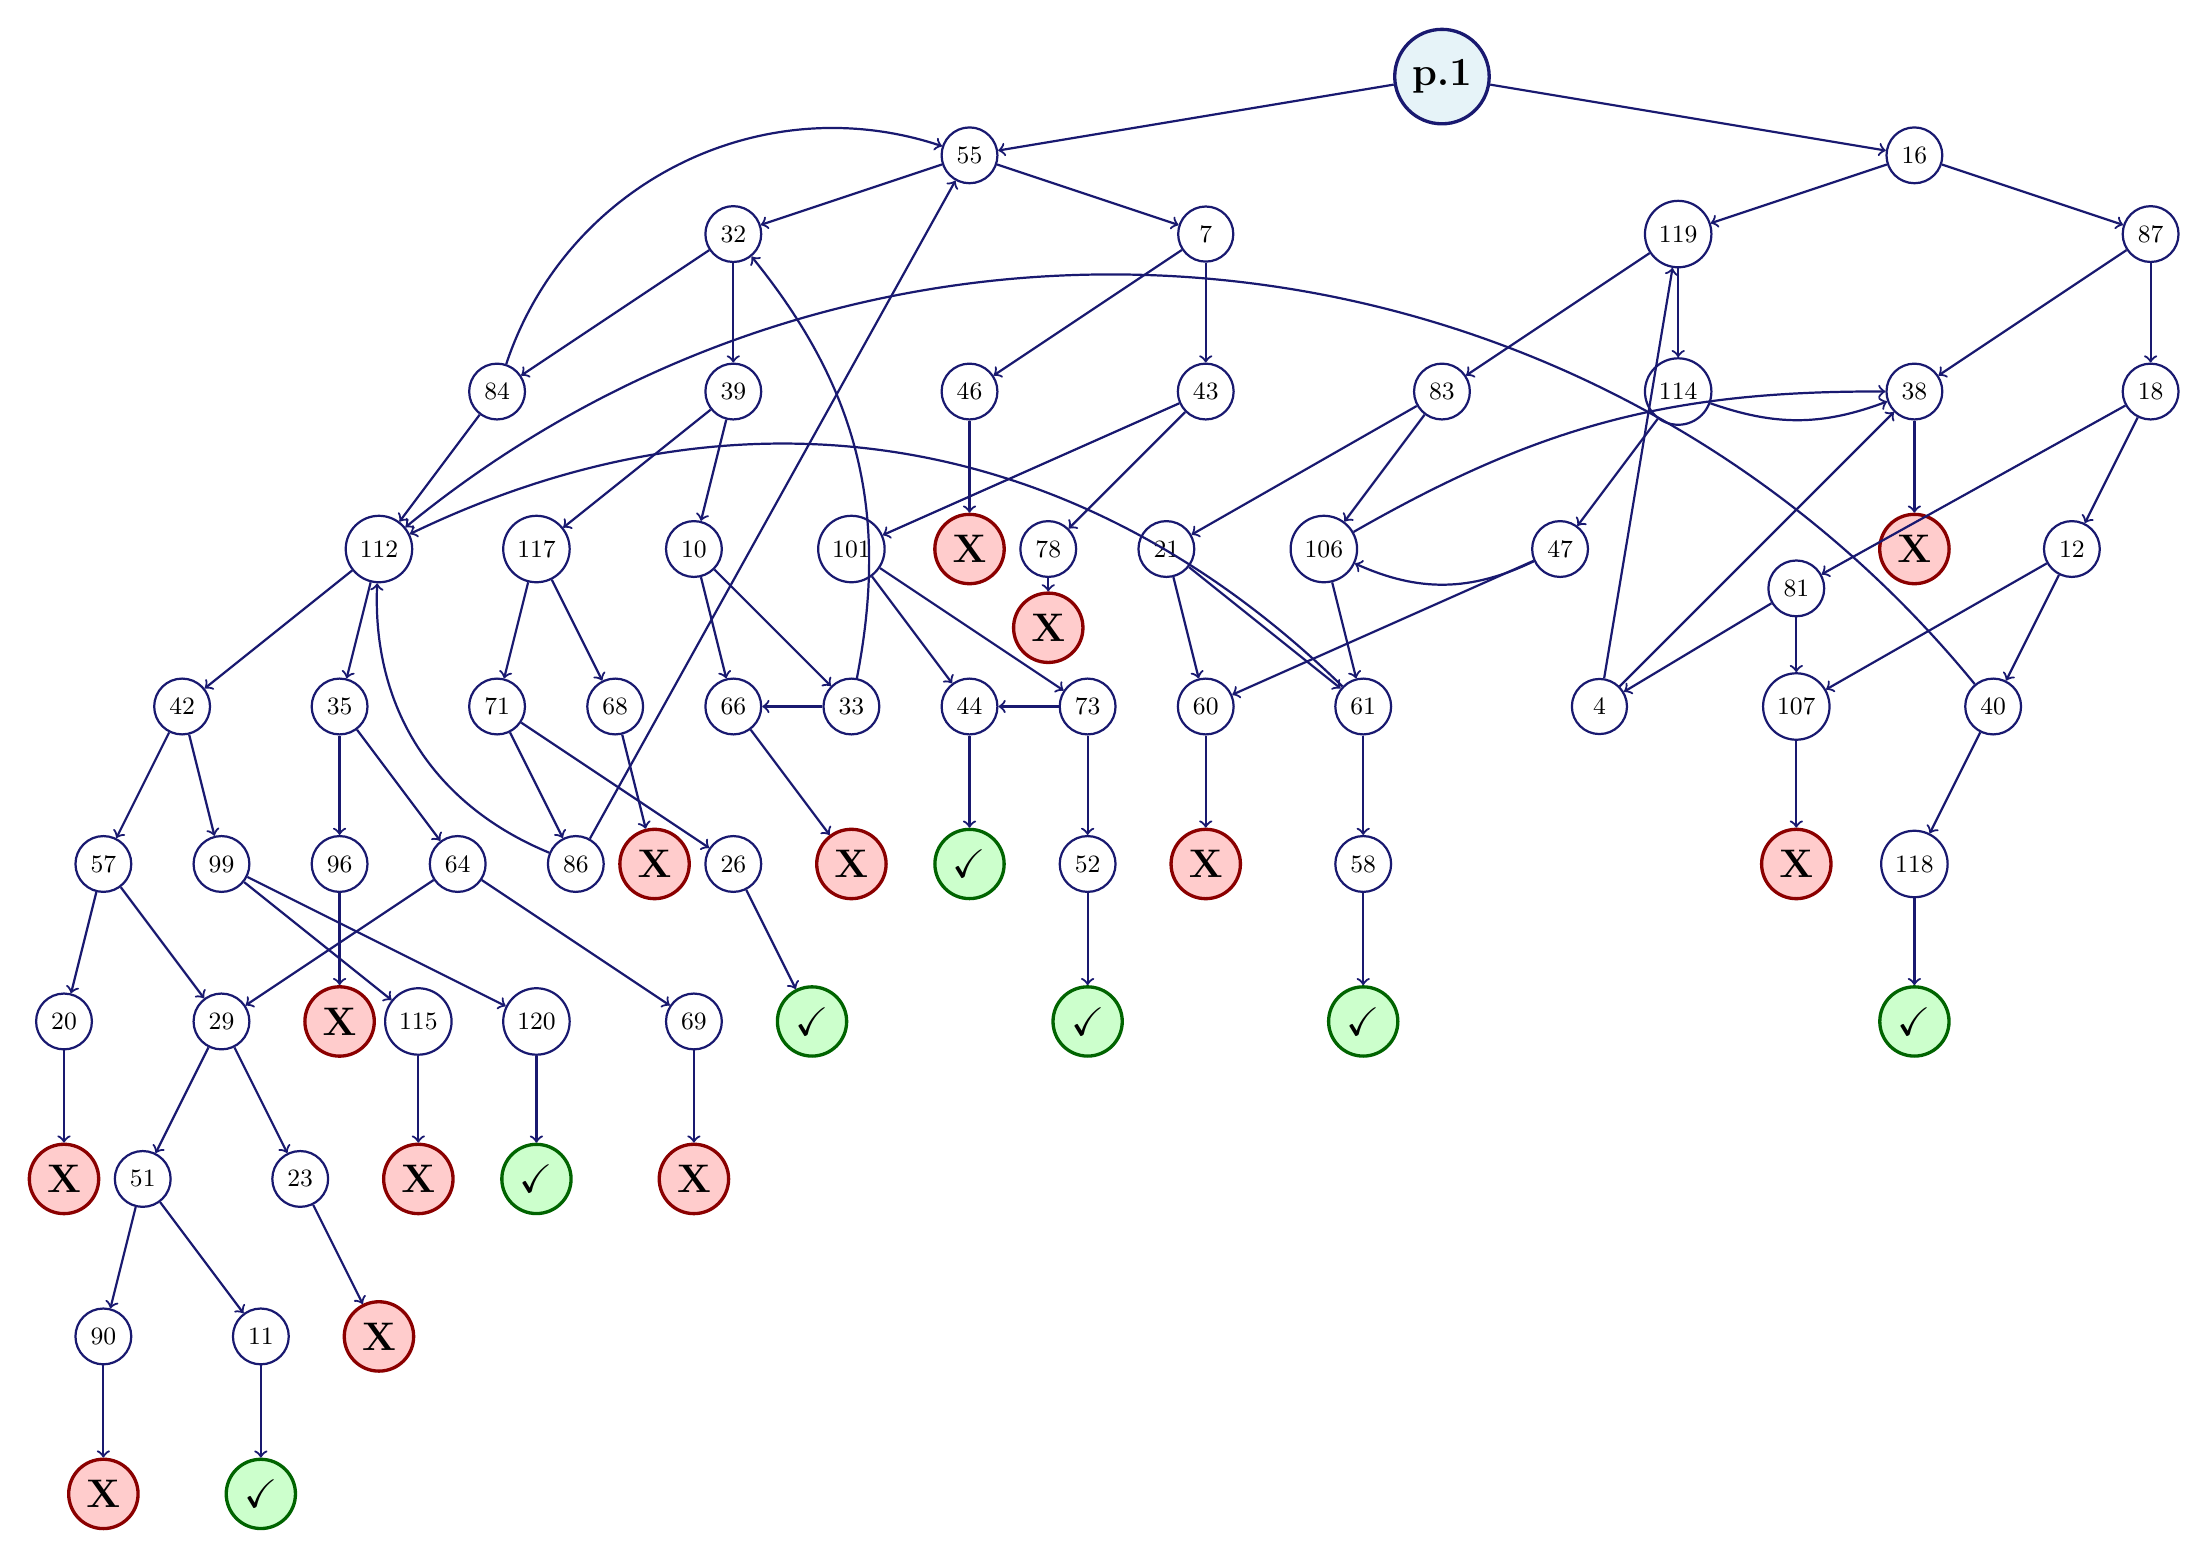
\begin{tikzpicture}[
    % Node styles
    start/.style={circle, draw=darkblue, fill=lightblue!30, minimum size=12mm, very thick, font=\Large\bfseries},
    page/.style={circle, draw=darkblue, minimum size=7mm, thick, font=\small},
    success/.style={circle, draw=darkgreen, fill=green!20, minimum size=7mm, very thick, font=\Large\bfseries},
    failure/.style={circle, draw=darkred, fill=red!20, minimum size=7mm, very thick, font=\Large\bfseries},
    % Edge styles
    edge/.style={draw=darkblue, thick, ->},
    backedge/.style={draw=darkblue, thick, ->}
]

% Level 0 - Start
\node[start] (p1) at (0,0) {p.1};

% Level 1
\node[page] (p55) at (-6,-1) {55};
\node[page] (p16) at (6,-1) {16};

% Level 2
\node[page] (p32) at (-9,-2) {32};
\node[page] (p7) at (-3,-2) {7};
\node[page] (p119) at (3,-2) {119};
\node[page] (p87) at (9,-2) {87};

% Level 3
\node[page] (p84) at (-12,-4) {84};
\node[page] (p39) at (-9,-4) {39};
\node[page] (p46) at (-6,-4) {46};
\node[page] (p43) at (-3,-4) {43};
\node[page] (p83) at (0,-4) {83};
\node[page] (p114) at (3,-4) {114};
\node[page] (p38) at (6,-4) {38};
\node[page] (p18) at (9,-4) {18};

% Level 4
\node[page] (p112) at (-13.5,-6) {112};
\node[page] (p117) at (-11.5,-6) {117};
\node[page] (p10) at (-9.5,-6) {10};
\node[page] (p101) at (-7.5,-6) {101};
\node[page] (p78) at (-5,-6) {78};
\node[page] (p21) at (-3.5,-6) {21};
\node[page] (p106) at (-1.5,-6) {106};
\node[page] (p47) at (1.5,-6) {47};
\node[page] (p81) at (4.5,-6.5) {81};
\node[page] (p12) at (8,-6) {12};

% Level 5
\node[page] (p42) at (-16,-8) {42};
\node[page] (p35) at (-14,-8) {35};
\node[page] (p71) at (-12,-8) {71};
\node[page] (p68) at (-10.5,-8) {68};
\node[page] (p66) at (-9,-8) {66};
\node[page] (p33) at (-7.5,-8) {33};
\node[page] (p44) at (-6,-8) {44};
\node[page] (p73) at (-4.5,-8) {73};
\node[page] (p60) at (-3,-8) {60};
\node[page] (p61) at (-1,-8) {61};
\node[page] (p4) at (2,-8) {4};
\node[page] (p107) at (4.5,-8) {107};
\node[page] (p40) at (7,-8) {40};

% Level 6
\node[page] (p57) at (-17,-10) {57};
\node[page] (p99) at (-15.5,-10) {99};
\node[page] (p96) at (-14,-10) {96};
\node[page] (p64) at (-12.5,-10) {64};
\node[page] (p86) at (-11,-10) {86};
\node[page] (p26) at (-9,-10) {26};
\node[page] (p52) at (-4.5,-10) {52};
\node[page] (p58) at (-1,-10) {58};
\node[page] (p118) at (6,-10) {118};

% Level 7
\node[page] (p20) at (-17.5,-12) {20};
\node[page] (p29) at (-15.5,-12) {29};
\node[page] (p115) at (-13,-12) {115};
\node[page] (p120) at (-11.5,-12) {120};
\node[page] (p69) at (-9.5,-12) {69};

% Level 8
\node[page] (p51) at (-16.5,-14) {51};
\node[page] (p23) at (-14.5,-14) {23};

% Level 9
\node[page] (p90) at (-17,-16) {90};
\node[page] (p11) at (-15,-16) {11};

% Success nodes (at various levels)
\node[success] (win11) at (-15,-18) {$\checkmark$};
\node[success] (win26) at (-8,-12) {$\checkmark$};
\node[success] (win44) at (-6,-10) {$\checkmark$};
\node[success] (win52) at (-4.5,-12) {$\checkmark$};
\node[success] (win58) at (-1,-12) {$\checkmark$};
\node[success] (win118) at (6,-12) {$\checkmark$};
\node[success] (win120) at (-11.5,-14) {$\checkmark$};

% Failure nodes (at various levels)
\node[failure] (fail20) at (-17.5,-14) {X};
\node[failure] (fail23) at (-13.5,-16) {X};
\node[failure] (fail38) at (6,-6) {X};
\node[failure] (fail46) at (-6,-6) {X};
\node[failure] (fail60) at (-3,-10) {X};
\node[failure] (fail66) at (-7.5,-10) {X};
\node[failure] (fail68) at (-10,-10) {X};
\node[failure] (fail69) at (-9.5,-14) {X};
\node[failure] (fail78) at (-5,-7) {X};
\node[failure] (fail90) at (-17,-18) {X};
\node[failure] (fail96) at (-14,-12) {X};
\node[failure] (fail107) at (4.5,-10) {X};
\node[failure] (fail115) at (-13,-14) {X};

% Draw regular forward edges (Level 0-1)
\draw[edge] (p1) -- (p55);
\draw[edge] (p1) -- (p16);

% Level 1-2
\draw[edge] (p55) -- (p32);
\draw[edge] (p55) -- (p7);
\draw[edge] (p16) -- (p119);
\draw[edge] (p16) -- (p87);

% Level 2-3
\draw[edge] (p32) -- (p84);
\draw[edge] (p32) -- (p39);
\draw[edge] (p7) -- (p46);
\draw[edge] (p7) -- (p43);
\draw[edge] (p119) -- (p83);
\draw[edge] (p119) -- (p114);
\draw[edge] (p87) -- (p38);
\draw[edge] (p87) -- (p18);

% Level 3-4
\draw[edge] (p84) -- (p112);
\draw[edge] (p39) -- (p117);
\draw[edge] (p39) -- (p10);
\draw[edge] (p46) -- (fail46);
\draw[edge] (p43) -- (p101);
\draw[edge] (p43) -- (p78);
\draw[edge] (p83) -- (p21);
\draw[edge] (p83) -- (p106);
\draw[edge] (p114) -- (p47);
\draw[edge] (p38) -- (fail38);
\draw[edge] (p18) -- (p81);
\draw[edge] (p18) -- (p12);

% Level 4-5
\draw[edge] (p112) -- (p42);
\draw[edge] (p112) -- (p35);
\draw[edge] (p117) -- (p71);
\draw[edge] (p117) -- (p68);
\draw[edge] (p10) -- (p66);
\draw[edge] (p10) -- (p33);
\draw[edge] (p101) -- (p44);
\draw[edge] (p101) -- (p73);
\draw[edge] (p78) -- (fail78);
\draw[edge] (p21) -- (p60);
\draw[edge] (p21) -- (p61);
\draw[edge] (p106) -- (p61);
\draw[edge] (p47) -- (p60);
\draw[edge] (p81) -- (p4);
\draw[edge] (p81) -- (p107);
\draw[edge] (p12) -- (p107);
\draw[edge] (p12) -- (p40);

% Level 5-6
\draw[edge] (p42) -- (p57);
\draw[edge] (p42) -- (p99);
\draw[edge] (p35) -- (p96);
\draw[edge] (p35) -- (p64);
\draw[edge] (p71) -- (p86);
\draw[edge] (p71) -- (p26);
\draw[edge] (p68) -- (fail68);
\draw[edge] (p66) -- (fail66);
\draw[edge] (p33) -- (p66);
\draw[edge] (p44) -- (win44);
\draw[edge] (p73) -- (p44);
\draw[edge] (p73) -- (p52);
\draw[edge] (p60) -- (fail60);
\draw[edge] (p61) -- (p58);
\draw[edge] (p4) -- (p119);
\draw[edge] (p4) -- (p38);
\draw[edge] (p107) -- (fail107);
\draw[edge] (p40) -- (p118);

% Level 6-7
\draw[edge] (p57) -- (p20);
\draw[edge] (p57) -- (p29);
\draw[edge] (p99) -- (p115);
\draw[edge] (p99) -- (p120);
\draw[edge] (p96) -- (fail96);
\draw[edge] (p64) -- (p69);
\draw[edge] (p64) -- (p29);
\draw[edge] (p86) -- (p55);
\draw[edge] (p26) -- (win26);
\draw[edge] (p52) -- (win52);
\draw[edge] (p58) -- (win58);
\draw[edge] (p118) -- (win118);

% Level 7-8
\draw[edge] (p20) -- (fail20);
\draw[edge] (p29) -- (p51);
\draw[edge] (p29) -- (p23);
\draw[edge] (p115) -- (fail115);
\draw[edge] (p120) -- (win120);
\draw[edge] (p69) -- (fail69);

% Level 8-9
\draw[edge] (p51) -- (p90);
\draw[edge] (p51) -- (p11);
\draw[edge] (p23) -- (fail23);

% Level 9-terminal
\draw[edge] (p90) -- (fail90);
\draw[edge] (p11) -- (win11);

% Back edges (with special styling)
\draw[backedge] (p84) to[bend left=45] (p55);
\draw[backedge] (p33) to[bend right=25] (p32);
\draw[backedge] (p40) to[bend right=45] (p112);
\draw[backedge] (p47) to[bend left=25] (p106);
\draw[backedge] (p61) to[bend right=35] (p112);
\draw[backedge] (p86) to[bend left=35] (p112);
\draw[backedge] (p114) to[bend right=20] (p38);
\draw[backedge] (p106) to[bend left=15] (p38);

\end{tikzpicture}
}

% \vspace{0.5cm}

% \begin{minipage}{0.45\textwidth}
% {\large\bfseries Legend:}\\[0.2cm]
% \begin{itemize}
% \item \textcolor{darkblue}{Blue circles}: Story pages
% \item \textcolor{lightblue}{Light blue circle}: Start
% \item \textcolor{darkgreen}{Green $\checkmark$}: Success ending
% \item \textcolor{darkred}{Red X}: Failure ending
% \item Solid arrows: All paths (including loops)
% \end{itemize}
% \end{minipage}
% \begin{minipage}{0.5\textwidth}
% {\large\bfseries Statistics:}
% \begin{itemize}
% \item Total pages: 56
% \item Maximum depth: 10 levels
% \item Success paths: 7
% \item Failure paths: 14
% \item Loop edges: 13
% \end{itemize}
% \end{minipage}

\end{landscape}
\end{document}